\section{Sepsis}

Sepsis is a condition, that develops on behalf of Systemic inflammatory response syndrome (SIRS) with pressence of an infection or bacteria in the tissue, within the body which triggers an immune response. This response often overexposures the workload on the immune system to fight the inflammation or bacteria. The infection or bacteria can be anywhere in the body’s tissue. Some of the normal macrohaemodynamics of sepsis are abnormal body temperature, abnormal heart rate, oxygen extraction and abnormal blood pressure \cite{plunta2010,kanta2014}. Sepsis is increasing condition in the population. Different studies suggest estimates of the incidence of sepsis, but the identification of diagnosis of sepsis can vary, why the numbers may also vary from place to place. The North American Centers for Disease Control found an increase in sepsis incidence pr. 100 000 patients, from 73.6 in 1979 to 175.9 in 1989, which is an increase of 82\% in 10 years \cite{baudouin2008,kanta2014}. The Dr Foster Organisation found an increase by 53\% from 1996 to 2002 in the hospitals in the United Kingdom. Causes for the increase in incidence can be due to the increasing elderly population, with cronic conditions undergoing invasive procedures \cite{baudouin2008}.
Sepsis is often assosiated with three stages, sepsis, severe sepsis and septic shock. This is illustrated in figure \ref{fig:Sepsis_stages}.

\begin{figure}[H]
	\centering	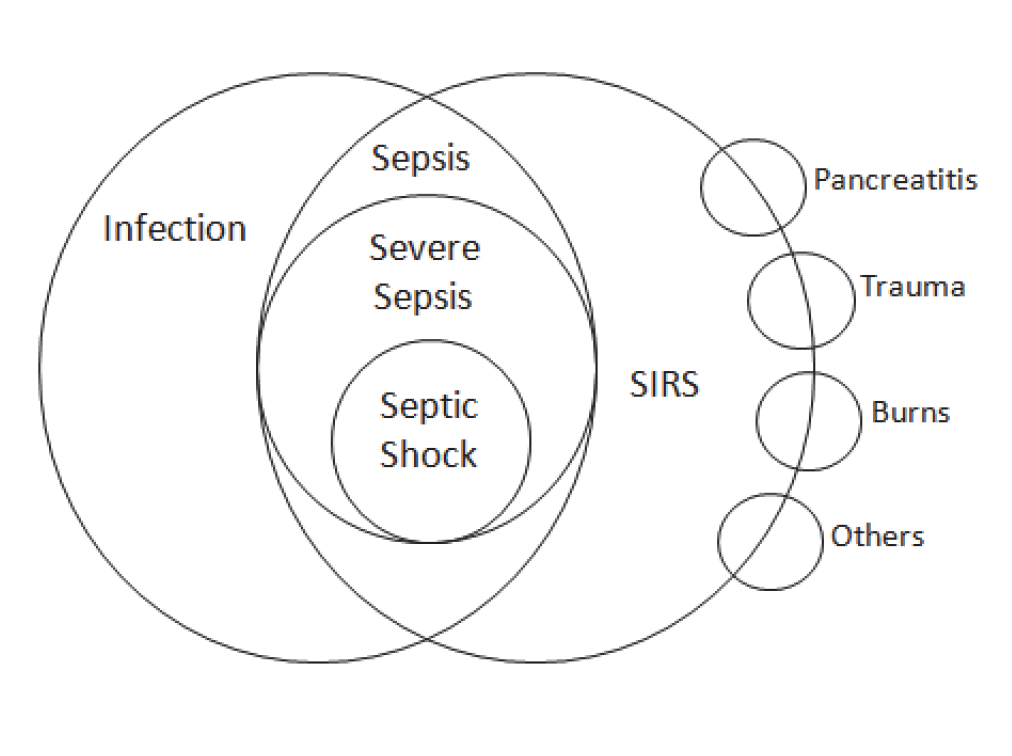
\includegraphics[width=0.65\textwidth]{figures/Sepsis_stages}
	\caption{Relation between SIRS and infectoin. Showing the stages in sepsis and some of the causes of SIRS which include pancreatitis, trauma, burns etc.}
	\label{fig:Sepsis_stages}
\end{figure} \vspace{-.3cm}

\subsection{Sepsis}

Under the condition of sepsis several things happen, mainly to the micro circulatory system at the capillary level, that leads to impaired homeostasis in the body. Infection or other bacteria that’s responsible for causing some irregularity is present in the blood and in the tissues around the the vessels. Among the first thing’s that happens when the body encounters an infection, white blood cells are recruited to release molecules that will fight the infection. Molecules that interact with the endothelial in the blood vessels, like nitric oxide (NO), are released. The interaction causes the vessels to dilate to increase the blood vessel diameter and permeability. The increased diameter slows down the blood flow, which causes a drop in blood pressure. Also the vessels permeability is increased. This reaction happens multiple places in the body where there is infected tissue present and will cause systemically vessel dilation. The characterization of sepsis is SIRS as a result of infection. \cite{baudouin2008,kanta2014}

\subsection{Severe sepsis}

When the permeability of the vessels is increased there will be more fluid in the tissue and the cells will get less oxygen because the oxygen has a harder time to get to the demanding tissue. Also the endothelial of the vessels will get damaged when the white blood cells try to destroy the pathogens. This triggers coagulation and clotting is formed in the damaged areas in the blood vessels. These clots can break off into the blood and cause further harm. At a point the damaged vessels leads to more leakage, because there will be a point where the coagulation can’t follow up. Organs will start to dysfunction at this stage. The characterization of severe sepsis is presence of sepsis with organ dysfunction and hypoperfusion is often included in this state. The mortality rate for patients with severe sepsis are about 25 to 30\% \cite{baudouin2008,kanta2014}. 

\subsection{Septic shock}

Septic shock happens when the body has undergone sepsis for a greater duration of time. This stage is characterized by a condition with hypotension even after adequate fluid resuscitation is given. Because of lactic acidosis the cells are not getting a sufficient supply of oxygen and therefore the cells will begin to die. This can lead to a very dangerous state, where organs begin to fail because they get to damaged to function. When multiple organs get damaged the state in septic shock reaches multiple organ failure also called multiple organ dysfunction syndrome (MODS)\cite{baudouin2008,kanta2014}. The mortality for patients with septic shock are in the region of 40 to 70\% \cite{kanta2014}. 

